\documentclass[12pt]{report}
\usepackage[lofdepth,lotdepth]{subfig}
\usepackage{graphicx}
\usepackage{verbatim}
\usepackage[utf8]{inputenc}
\usepackage[english,italian]{babel}
\usepackage{amsfonts}
\usepackage{color}
\usepackage{indentfirst}
\usepackage{makeidx}
\usepackage{listings}
\usepackage{fancyhdr}
\usepackage{amssymb}
\usepackage{textcomp}
\usepackage{caption}
\usepackage{url}
\setlength{\headheight}{15pt}
\lstset{postbreak=\space, breakindent=5pt, breaklines}

\date{}
\newcommand{\CB}{CIBIR}

% Per avere il bold typewriter
\DeclareFontShape{OT1}{cmtt}{bx}{n}{ <5><6><7><8><9><10><10.95><12><14.4><17.28><20.74><24.88>cmttb10}{}

\lstdefinestyle{c}{
	language=Java,
	basicstyle=\footnotesize,
	keywordstyle=\bfseries,
	identifierstyle=\ttfamily,
	stringstyle=\ttfamily,
	captionpos=b,
	abovecaptionskip=15pt,
	showstringspaces=false
}

\usepackage{amsmath}

\usepackage[top=5.5cm, bottom=2.5cm, left=4.5cm, right=3cm]{geometry}
\newcommand{\citazione}[1]{``#1''}
\makeindex

\begin{document}
\pagenumbering{Roman}
\begin{titlepage}
\begin{center}
\begin{figure}[!t]
\vspace{-3truecm}
\centering

\includegraphics[width=3cm]{img/unict.eps}
\end{figure}
\uppercase{Universit\`a degli Studi di Catania}\\
{\sc Dipartimento di Ingegneria Elettrica, Elettronica e Informatica}\\
{\sc corso di laurea magistrale in Ingegneria Informatica}\\
\hbox to \textwidth{\hrulefill}

\vspace{3truecm}

{\sc Silvia Sottile}

\vspace{2truecm}

 {\sc Progettazione e realizzazione di uno store per la Social Internet of Things basato su Blockchain}

\vspace{2truecm}

\centerline{\hbox to 3.5truecm{\hrulefill}}

{\sc Tesi di Laurea}

\centerline{\hbox to 3.5truecm{\hrulefill}}

\vspace{2truecm}

\begin{minipage}{\textwidth}
\begin{flushright}
\begin{minipage}{0.3\textwidth}
\begin{tabbing}
Relat\=ore:
\\Chiar.mo \=Prof. \= {\sc G. Morabito} \\
\\Correlatore: 
\\Ing.  \= {\sc S. Quattropani}\\

\end{tabbing}
\end{minipage}
\end{flushright}
\end{minipage}

\vspace{1truecm}

\hbox to \textwidth{\hrulefill}
{\sc Anno Accademico 2017/2018}

\end{center}
\end{titlepage}

\endinput
\bibliographystyle{unsrt}
 % frontespizio

\pagestyle{empty}
\null\vspace {\stretch {1}}
\begin {flushright}
\textit{Alla mia famiglia e a Sebastiano.}
\end {flushright}
\vspace {\stretch {2}}\null


\newpage

\pagestyle{plain}
\input{Capitoli/Abstract} %%%% METTERE ??
\newpage

\selectlanguage{italian}
\setlength{\baselineskip}{1.8\baselineskip} % interlinea

\tableofcontents
\listoffigures
\lstlistoflistings

\clearpage
\clearpage
\pagenumbering{arabic}
% Intestazione con fancy header, eliminato intestazione sinistra
\pagestyle{fancy}
\lhead{}

%%%%%%%%%%%%%%%%%%%%%%%%%%%%%%%%%%%%%%%%%%%%%%%%%%%%%%%%%%%%%%%%%%%%%%%%%%%%%%%%%%%%%%%%

\chapter*{Introduzione}
\label{c:intro}
Il paradigma dell'Internet of Things ha aperto la strada verso un mondo in cui i nostri oggetti di uso comune saranno interconnessi e interagiranno con l'ambiente esterno per raccogliere informazione e automatizzare alcuni task. Questa visione implica una serie di feature, come autenticazione, privacy dei dati, sicurezza, robustezza agli attacchi, sviluppo agevole delle applicazioni e self-maintenance.\cite{Fernandez-Carames2018}

Queste caratteristiche possono essere implementate attraverso l'uso della \textit{Blockchain}, una tecnologia nata insieme alla famosa criptovaluta \textit{Bitcoin}. 

%*** Puppette sulla blockchain ***

Questo lavoro di tesi si concentrerà sull'integrazione della blockchain in un sistema basato sulla Social Internet of Things, il GRIDS (Generic Resilient Identity Services) System, il quale permette di migliorare le operazioni di mapping ID-to-locator attraverso la navigazione del grafo SIoT creato dalle relazioni che si stabiliscono tra gli oggetti.

Il capitolo \ref{c:tec} parla dello stato dell'arte: per quanto riguarda l'Internet of Things, verrà fatta una veloce panoramica sulla sua evoluzione, con una particolare attenzione sul Social IoT, citando inoltre alcune piattaforme di virtualizzazione. Verranno presentate anche le caratteristiche principali della blockchain, portando come esempio la rete Bitcoin.... 

Ci sono anche elementi di crittografia, fondamentale per poter capire appieno il funzionamento della blockchain.....

Verrà introdotto il GRIDS System nel capitolo \ref{c:grids}, con particolare attenzione sull'architettura e sull'implementazione in Java....

Il capitolo \ref{c:integr} costituisce la parte centrale del lavoro: saranno illustrati i passi seguiti per l'integrazione della blockchain nel sistema, dalla scelta della blockchain stessa all'interfaccia grafica per l'interazione dell'utente con il sistema...

Il capitolo successivo si concentra sulla valutazione delle performance ....

Per concludere, verranno suggeriti dei potenziali sviluppi futuri che possano migliorare ulteriormente il sistema......
\newpage

%%%%%%%%%%%%%%%%%%%%%%%%%%%%%%%%%%%%%%%%%%%%%%%%%%%%%%%%%%%%%%%%%%%%%%%%%%%%%%%%%%%%%%%%

\chapter{Stato dell'Arte}
\label{c:tec} 
% ************
\section{Internet of Things}
\label{c:tec:iot}

La società odierna è sempre più permeata dalla presenza di Internet. La Rete è ormai diventata un bene fondamentale che, se dovesse all'improvviso scomparire, getterebbe nel panico la quasi totalità delle aziende e delle persone. In questo scenario, una tendenza che, da qualche anno a questa parte, sta prendendo piede è che le entità connesse a Internet non siano solo le persone (con i propri smartphone, personal computer ecc.), ma anche gli oggetti: si parla infatti di \textit{Internet of Things} (IoT). Elettrodomestici, sensori, attuatori, dispositivi elettronici di natura eterogenea che, dotati di una scheda di rete, hanno accesso a Internet e possono essere collegati tra loro per formare una rete interconnessa. Esso si riferisce non solo al fatto che gli oggetti possano collegarsi fra di loro, ma anche al fatto che sia esseri umani, sia oggetti fisici, sia ambienti e dati virtuali possono interagire tra di loro nello stesso tempo e spazio.

La forza di questa idea è il grande impatto che avrebbe sui diversi aspetti della vita quotidiana e anche sul comportamento dei potenziali utenti. Se si tratta di un privato, gli effetti dell'introduzione dell'IoT più evidenti sono visibili sia in ambiente lavorativo che in ambiente domestico. La domotica, l'e-health, l'apprendimento potenziato sono solo alcuni esempi delle possibili applicazioni in cui questo nuovo paradigma avrà un ruolo fondamentale nel prossimo futuro. In maniera simile, anche le aziende possono usufruire dell'IoT in campi come l'automazione, la logistica, gestione dei processi, trasporto intelligente di merci e persone. 
Per questi motivi l'Internet of Things può essere considerato, dopo la nascita del World Wide Web negli anni '90 e quella di Internet mobile nel 2000, come la frontiera di Internet potenzialmente più rivoluzionaria.

Le prime applicazioni dell'IoT, nei primissimi anni 2000, furono nel campo manifatturiero con l'impiego della tecnologia RFID (\textit{Radio Frequency IDentification}), attraverso la quale è possibile l'identificazione e la memorizzazione automatica di informazioni legate agli oggetti, consentendo cos\`i di poterli tracciare nel percorso dal centro di distribuzione agli scaffali dei negozi.

Alcuni anni dopo, nel pieno del progresso tecnologico, la diminuzione dell'area occupata dai chip e la riduzione dei consumi energetici, portò allo sviluppo di nuove tecnologie. Un esempio molto importante, che deriva direttamente dai tag RFID, era la tecnologia \textit{Near Field Communication} (NFC), che fornisce connettività wireless a corto raggio con comunicazione bidirezionale.

Un altro importante passo per lo sviluppo dell'IoT fu la creazione delle prime \textit{Wireless Sensor Network} (WSN). Una rete WSN è costituita da un insieme di nodi sensori o \textit{sensor nodes}, cioè componenti in grado di rilevare grandezze fisiche (come la posizione, la temperatura, l'umidità, la luce, o anche il movimento di veicoli, la composizione del terreno, livello di rumore ecc.), di elaborare dati e di comunicare tra loro. I nodi sensore all'interno di una rete hanno la possibilità di collaborare tra loro, dal momento che sono provvisti di un processore on-board; grazie a quest'ultimo, ciascun nodo, invece di inviare dati grezzi ai nodi responsabili della raccolta dei dati, può effettuare delle semplici elaborazioni e trasmettere solo i dati richiesti e già elaborati, cosa che con l'RFID non era possibile. 

Con il passare del tempo, il numero di dispositivi attivi cresceva esponenzialmente di anno in anno, e in più la creazione di reti e protocolli di comunicazione ad hoc per gli oggetti (proprio come nel caso dei sistemi RFID) diventava sempre più superflua in un'epoca in cui Internet, con il suo stack protocollare TCP/IP, si diffondeva a macchia d'olio: l’esigenza che nacque, quindi, era quella di trasformare gli oggetti in semplici nodi di Internet. In altre parole, dovevano possedere un indirizzo IP e usare l'Internet Protocol per comunicare con gli altri oggetti e con gli altri nodi della rete.

Gli oggetti, grazie a questo, diventano \textit{smart objects}, e possono quindi utilizzare i servizi e le applicazioni già esistenti, come il protocollo a livello applicazione HTTP, e diventare effettivi partecipanti non solo di Internet, ma del World Wide Web. 

Un problema che subito si presentava, tuttavia, era la limitata disponibilità di risorse degli \textit{smart objects}, come le capacità computazionali dei processori e i consumi energetici, e quindi dei costi. Uno standard di comunicazione wireless per i livelli 1 e 2 dello stack di comunicazione che presenta consumi relativamente bassi è l'IEEE 802.15.4, conosciuto come \textit{ZigBee}, e venne creato un nuovo protocollo per il livello 3 che si adattava alle caratteristiche di quest'ultimo: è il caso dell'\textit{IPv6 over Low Power Wireless Area Networks} (6LoWPAN).

L'interesse verso questo nuovo standard di comunicazione è cresciuto notevolmente, tanto che sono stati definiti altri protocolli per gli altri livelli dello stack. Un esempio importante è il \textit{Constrained Application Protocol} (CoAP): esso è un protocollo a livello applicazione adatto all’interazione tra dispositivi chiamati, per l'appunto, \textit{constrained}, cioè dalle risorse hardware limitate.

Protocolli come quest'ultimo hanno permesso la formazione dell'insieme di approcci e pattern di programmazione chiamato \textit{Web of Things} (WoT), il quale consente agli oggetti del mondo reale di prendere parte non solo ad Internet, ma al World Wide Web.


%%%%%%%%%%%%%%%%%%%%%
\subsection{Social IoT}
\label{c:tec:siot}
Un'evoluzione che l'IoT ha sub\`ito in tempi molto recenti è l'introduzione del concetto di \textit{social networking} nella sua architettura, formando il cosiddetto \textit{Social Internet of Things}\cite{Atzori2012} (SIoT), che consiste in una rete in cui gli oggetti possono formare delle relazioni e interagire tra loro senza il diretto intervento umano. Questo fenomeno è dovuto ai grandi vantaggi che si verrebbero a creare con questo nuovo paradigma: la navigabilità della rete, che diventa molto più facile, permettendo la ricerca di servizi specifici in modi efficienti; l'introduzione di diversi gradi di affidabilità per regolare il grado di interazione tra oggetti con tipi di relazioni diverse, per avere un certo livello di sicurezza; il riutilizzo dei modelli di studio dei social network per risolvere problemi relativi all'IoT, come la grande estensione della rete di oggetti interconnessi tra loro; la possibilità di stabilire relazioni tra oggetti che usano differenti tecnologie, cosa molto importante per permettere l'interazione tra diverse piattaforme per IoT. In questo scenario, quindi, si può immaginare un mondo popolato da oggetti intelligenti che permeano la vita quotidiana degli esseri umani.

Tuttavia, solo pochi dispositivi IoT hanno le capacità computazionali per poter creare e gestire le relazioni sociali: diventa, quindi, di fondamentale importanza il cloud computing, con il quale è possibile virtualizzare gli oggetti per consentire l'esecuzione, il deployment e il provisioning delle applicazioni. Per implementare il Social IoT, quindi, è necessario impiegare un modello che funga da controparte virtuale degli oggetti fisici, che viene eseguito sui server del cloud, chiamato Social Virtual Object. Le caratteristiche che una piattaforma per il SIoT dovrebbe avere per fornire un buon servizio sono le seguenti:
\begin{itemize}
\item una bassa latenza nel collegamento tra oggetto fisico e corrispettivo digitale;
\item scalabilità, per far fronte al traffico generato dall'enorme numero di dispositivi potenzialmente collegabili;
\item dei social agent autonomi che permettano ai nodi IoT dalle risorse limitate a mantenere e aggiornare le relazioni sociali in maniera consistente;
\item gestione della mobilità, per fornire servizi che si basano sulla posizione dei dispositivi e per consentire la migrazione dei SVO attraverso i server cloud distribuiti geograficamente.
\end{itemize}

Le relazioni che gli oggetti possono stabilire sono le seguenti: la \textit{Ownership Object Relationship} (OOR) si crea tra oggetti appartenenti allo stesso proprietario, la \textit{Co-location Object Relationship} (CLOR) tra dispositivi che si trovano nello stesso luogo, come per esempio gli elettrodomestici di un'abitazione, la \textit{Parental Object Relationship} (POR) tra oggetti che hanno lo stesso modello, produttore e lotto di produzione, la \textit{Co-work Object Relationship} (CWOR) tra oggetti che si incontrano nel luogo di lavoro del proprietario, come ad esempio il computer e la stampante dell'ufficio, infine la \textit{Social Object Relationship} (SOR) tra oggetti che si trovano spesso vicini tra loro, come per esempio gli smartphone delle persone che si trovano ogni giorno sullo stesso autobus per andare al lavoro o a scuola.

Inoltre, possono essere usati due diversi approcci per la costruzione delle reti di oggetti del Social IoT: il primo è quello del Social Web of Things, in cui viene costruito un ecosistema che consente alle persone e agli smart objects di interagire tra di loro all'interno di un unico framework. In questo caso le tecnologie web vengono utilizzate per fornire dei servizi ai nodi della rete. Un secondo approccio, più restrittivo, è rappresentato dal Social Internet of Things in senso stretto, in cui gli oggetti formano legami autonomamente tra loro e sono separati dalle comunità virtuali formate dagli esseri umani, ai quali gli oggetti sono soltanto subordinati.

Sociologicamente la portata di questo cambiamento è molto importante per l'ipotetico spostamento di un paradigma interpretativo che pone al centro proprio l'uomo: macchine al servizio dell'uomo che comunicano con l'uomo.

%%%%%%%%%%%%%%%

\subsection{Piattaforme di virtualizzatione dei nodi IoT}
\label{c:tec:virt}

Le piattaforme di virtualizzazione permettono di ampliare le capacità computazionali dei IoT, dal momento che questi ultimi non sono generalmente dotati di grandi risorse hardware che permettono di immagazzinare la grande quantità di dati generati. Qui di seguito sono illustrate le due piattaforme utilizzate nel sistema, Thingspeak e Festival.

\paragraph{Thingspeak}
\label{c:tec:virt:ts}

Thingspeak è una piattaforma di virtualizzazione open-source realizzata da ioBridge nel 2010. Essa fornisce una serie di applicazioni e di API per poter raccogliere i dati generati dai nodi IoT e poterli processare attraverso il servizio di cloud. Questi vengono poi raccolti in un \textit{channel}, l'elemento primario della piattaforma, dal quale possono essere analizzati, visualizzati, calcolati nuovi dati e possono anche interagire con altri servizi web, come ad esempio i social media e altri dispositivi. Essa fornisce accesso a una grande varietà di dispositivi integrati, come Arduino, Raspberry Pi e BeagleBone Black. 

Thingspeak è open-source, cioè il suo codice sorgente e la lista completa delle API è interamente scaricabile e consultabile dai programmatori di tutto il mondo su GitHub.

Il suo funzionamento si basa su tre principali azioni:

\begin{itemize}
    \item Raccogliere i dati: vengono raccolti tutti quelli provenienti dai vari tipi di sensori (temperatura, pressione, umidità, campo magnetico ecc.), anche sotto forme diverse, come ad esempio valori numerici o segnali elettrici, e vengono inviati nello spazio di cloud riservato al canale.
    \item Analizzare i dati: una volta nel cloud, si possono utilizzare tool di analisi per visualizzare, scoprire relazioni, trend e pattern nei dati. Ciò è possibile grazie alla collaborazione di Thingspeak con \textit{Mathworks}, il quale fornisce gli strumenti di analisi di MATLAB agli utenti della piattaforma senza il bisogno dell’acquisto di una licenza. È possibile convertire, combinare e calcolare nuovi dati, pianificare l’esecuzione di calcoli in momenti ben precisi, usare funzioni built-in per creare grafici, combinare i dati provenienti da più canali analisi più sofisticate. 
    \item Agire sui dati: con l’applicazione \textit{TalkBack}, ad esempio, possono essere innescate delle reazioni al verificarsi di certi eventi, come ad esempio ricevere un tweet quando la temperatura rilevata da un certo sensore supera un determinato valore di gradi Celsius, oppure eseguire operazioni più complesse come azionare un motore. È possibile, quindi, far comunicare i dispositivi collegati alla piattaforma e anche mettere in fila dei comandi da far eseguire a ogni dispositivo. Con questa e con le altre applicazioni presenti nella piattaforma, quindi, è possibile automatizzare e pianificare azioni sia sui dispositivi fisici, sia sul web.
\end{itemize}

\paragraph{Festival}
\label{c:tec:virt:fest}

FESTIVAL è un progetto collaborativo tra Europa e Giappone facente parte di Horizon2020. Esso mira a rendere interoperabili dei testbed eterogenei, appartenenti alle categorie \textit{Open Data} (per esempio dataset), \textit{IoT} (per esempio sensori e attuatori), \textit{IT} (come risorse computazionali) e \textit{Living Labs} (ad esempio persone), per costruire un modello \textit{Experimentation as a Service} (EaaS).

FESTIVAL fornisce anche un insieme di funzionalità per gestire e monitorare gli esperimenti. La piattaforma è stata testata su tre domini di smart city dislocati tra Europa e Giappone: \textit{smart energy}, \textit{smart building} e \textit{smart shopping}.

Per l'implementazione della piattaforma è stato utilizzato il modello EaaS (Experiment as a Service), che permette agli sviluppatori di creare esperimenti replicabili e scalabili e di avere accesso a diversi testbed in maniera trasparente e omogenea. Fornisce inoltre funzionalità di discovery, le quali consentono di trovare le risorse con i requisiti necessari per gli esperimenti e le abilità per analizzare i risultati raccolti durante tutte le fasi degli esperimenti.

L'architettura di FESTIVAL è composta da due livelli: il primo organizza le risorse per categoria, chiamato \textit{“resource-based” federation}, mentre il secondo fornisce accesso a queste ultime (\textit{“experiment-based” federation}), come è possibile osservare in figura \ref{f:tec:festival}.

\begin{figure}[h!t]
\centerline{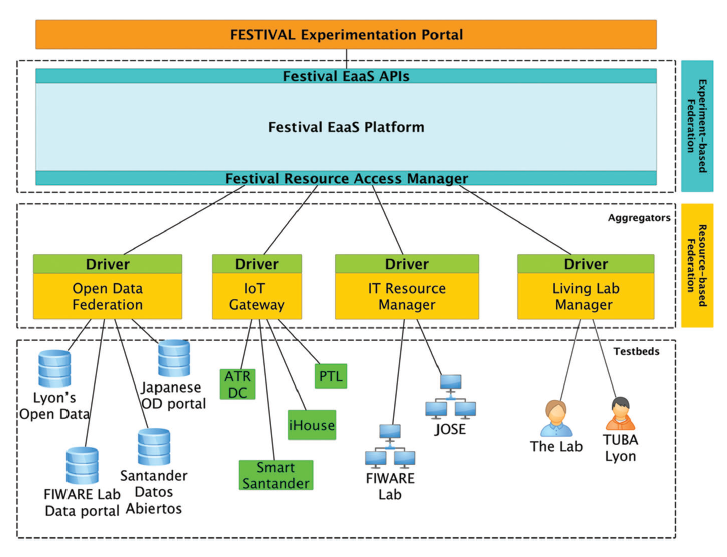
\includegraphics[scale=0.5]{img/festival}}
\caption{Architettura di FESTIVAL}
\label{f:tec:festival}
\end{figure}

Al di sotto di questi livelli è possibile vedere tutti i testbed coinvolti nel progetto, classificati secondo le seguenti tipologie: Open Data, IoT, IT e Living Lab. 

Il livello resource-based fornisce le funzionalità per l'integrazione di ciascun tipo di risorse, utilizzando componenti ad-hoc chiamati Aggregators. Ognuno di questi è indipendente dalla piattaforma, e serve a raggruppare le risorse dello stesso tipo, fornendo un modello dati e una descrizione uniformi. FESTIVAL supporta i seguenti Aggregator:
\begin{itemize}
    \item \textit{Open Data Federation}: esso serve a raggruppare i differenti \textit{Open Data Management Systems} (ODMS), fornendo le funzioni per cercare e per eseguire query sugli open data;
    \item \textit{IoT Gateway}: questo componente è necessario per fornire accesso ai dispositivi IoT, come sensori o smart objects, con i differenti protocolli IoT;
    \item \textit{IT Resource Manager}: esso raggruppa le risorse computazionali, e in particolare è responsabile della gestione di tutti gli aspetti legati alla prenotazione e accesso alle macchine virtuali;
    \item \textit{Living Lab Manager}: questo componente è in grado di raggruppare i living labs, considerando i servizi, metodologie ed esperienza dei loro membri come risorse che possono essere impiegate in un esperimento.  
\end{itemize}

Tutte le funzionalità a livello EaaS sono accessibili da applicazioni esterne attraverso un set di API. FESTIVAL, in particolare, fornisce un'applicazione web progettata per facilitare gli sviluppatori a gestire i propri esperimenti.


% ************
\section{Crittografia: cifratura asimmetrica}
\label{c:tec:cifratura}

La cifratura a chiave simmetrica è un meccanismo secondo il quale la stessa chiave viene utilizzata sia per cifrare che per decifrare; è molto intuitiva, dal momento che è un concetto molto vicino alla nostra quotidianità, l'aprire e chiudere una porta con la stessa chiave.
Questa caratteristica richiede meccanismi sofisticati per distribuire la chiave alle parti che comunicano in maniera sicura, visto che una volta scoperta la chiave di cifratura l'intera comunicazione è compromessa.

La cifratura asimmetrica, invece, introduce il concetto di avere non una, ma due chiavi: una per cifrare, l'altra per decifrare\cite{Cgi2004}. Questo meccanismo presenta molti vantaggi rispetto alla cifratura a chiave simmetrica:
\begin{itemize}
    \item distribuzione delle chiavi semplificata;
    \item \textit{Digital Signature};
    \item cifratura a lungo termine.
\end{itemize}

Ad ogni modo, la cifratura \textit{symmetric key} rimane ancora il principale metodo di implementazione delle \textit{Public-key Infrastructure} (PKI).

La componente principale della cifratura asimmetrica è la coppia di chiavi: una \textit{public key} e una \textit{private key}. La prima viene resa pubblica e quindi distribuita liberamente, mentra la seconda deve essere mantenuta segreta e mai distribuita. 

Dato un paio di chiavi, i dati che vengono cifrati con la public key possono essere decifrati solo con la private key, mentre i dati cifrati con la chiave privata vengono decifrati con la chiave pubblica. Questi meccanismi vengono utilizzati per realizzare, rispettivamente:
\begin{enumerate}
    \item \textit{Confidentiality} (solo il possessore della private key può leggere i dati cifrati con la chiave pubblica corrispondente). La cifratura è un meccanismo per cui un messaggio viene trasformato in modo tale da poter essere letto da mittente e destinatario. Per esempio, si supponga che Alice voglia inviare un messaggio a Bob. Per farlo, ha bisogno la chiave pubblica di Bob; visto che lui può mandarla attraverso la rete senza problemi, Alice cifra il messaggio utilizzando questa public key e lo manda a Bob. Egli riceve il messaggio e, utilizzando la sua chiave privata, è in grado di decifrarlo.
    \item \textit{Integrity} e \textit{authentication} attraverso la firma digitale: è un meccanismo per cui un messaggio viene autenticato, per esempio provando che proviene effettivamente da un certo mittente, proprio come una firma in un documento cartaceo. Per esempio, supponendo che Alice voglia apporre una firma digitale a un messaggio diretto a Bob. Per fare ciò, utilizza la propria private key per cifrare il messaggio e poi invia il messaggio cifrato con in più la propria chiave pubblica. Dal momento che la sola chiave che può decrittare il messaggio è la chiave pubblica di Alice, una decifratura che va a buon fine rappresenta una \textit{Digital Signature Verification}, cioè è la prova inconfutabile che il messaggio è stato cifrato con la chiave privata di Alice.
\end{enumerate}

% ************

\section{Blockchain e Bitcoin}
\label{c:tec:blockchain}

Una blockchain è un database distribuito che contiene record di un \textit{public ledger} (libro mastro) di tutte le transazioni o eventi digitali che sono stati eseguiti e condivisi tra le parti che vi partecipano. Ogni transazione nel public ledger viene verificata dal \textit{consenso} della maggioranza dei partecipanti nel sistema. E, una volta dentro, l'informazione non può più essere cancellata. La blockchain contiene un record verificabile di ogni singola transazione che sia stata mai fatta.

Per usare una metafora, è più facile rubare un biscotto da una scatola tenuta in un luogo nascosto rispetto a rubarlo da una scatola che si trova in piena vista in un supermercato davanti a migliaia di persone.

\textit{Bitcoin} è l'esempio di utilizzo della tecnologia della blockchain più famoso, ma anche più controverso, dato che rende possibili transazioni multimiliardarie nel mercato globale che sono totalmente anonime e fuori da ogni controllo delle autorità \cite{Nakamoto2008} \cite{BitcoinProject2014}. 

In ogni caso, la Blockchain di per sè non è per niente controversa, ed è stata impiegata in applicazioni sia finanziarie che non finanziarie con risultati impeccabili. Il modello di consenso distribuito della blockchain è stato addirittura incluso tra le invenzioni più rivoluzionarie dall'invenzione di Internet stesso da Marc Andreessen, uno dei più importanti imprenditori della Silicon Valley \cite{Crosby2016}.

L'economia digitale odierna si affida a delle \textit{trusted authority} per praticamente qualsiasi cosa: tutte le nostre transazioni online si basano sul fatto che esiste qualcuno che ci dice cosa è vero, ad esempio come un provider di un servizio email che ci dice che la nostra email è stata inviata; o come un social network che ci oppure come una banca che ci conferma che i nostri soldi sono stati inviati in maniera sicura ai nostri cari in un'altra nazione. In sostanza, viviamo precariamente la nostra vita digitale perch\'e contiamo su queste terze parti per la sicurezza e privacy dei nostri beni digitali. Il problema principale, però, è che queste possono essere hackerate e compromesse in qualche modo.

È proprio qui che la blockchain viene in aiuto: essa ha il potenziale per rivoluzionare il mondo digitale consentendo di raggiungimento di un consenso distribuito in cui qualsiasi transazione che coinvolga beni digitali può essere verificata in qualsiasi momento, senza compromettere la privacy dei beni e delle parti in questione. 

\subsection{Funzionamento}
\label{c:tec:blockchain:funzionamento}

Per spiegare i concetti alla base dalla blockchain è doveroso portare in esempio il funzionamento del sistema dei Bitcoin, dato che sono entrambi interconnessi. Ciò non toglie che la blockchain sia applicabile in qualsiasi altro ambito e bene digitale che viene scambiato online.

Il commercio su Internet è esclusivamente legato al fatto che le istituzioni finanziarie fungono da terza parte, la quale processa e media qualsiasi transazione elettronica. Il ruolo di una terza parte \textit{trusted} è quello di validare e salvaguardare le transazioni per evitare che avvengano frodi. Tutto ciò comporta alti costi.

Bitcoin, in un contesto in cui due parti vogliano eseguire una transazione su Internet, utilizza una prova crittografica invece della fiducia nella terza parte. Ogni transazione viene protetta da una firma digitale, cioè viene firmata con la \textit{private key} del mittente e poi inviata alla \textit{public key} del destinatario. Per poter spendere quei soldi, il proprietario della valuta deve dimostrare la proprietà della private key: per fare ciò, l'entità che riceve il denaro verifica la firma digitale della transazione utilizzando la public key del mittente.

Ogni transazione viene inviata in broadcast a tutti i nodi della rete Bitcoin e, dopo essere stata provata la sua validità, viene registrata in un \textit{public ledger} (libro mastro pubblico). Il nodo che effettua questa verifica deve assicurarsi che siano rispettati i seguenti requisiti:
\begin{enumerate}
    \item il mittente è il proprietario della firma digitale della transazione;
    \item il mittente possiede sufficiente criptovaluta nel suo account: bisogna cercare nel public ledger ogni transazione compiuta verso la sorgente della transazione (nello specifico la sua public key) per confermare che essa abbia credito sufficiente.
\end{enumerate}

Tuttavia, si presenta il problema del mantenimento dell'ordine delle transazioni che vengono diffuse nella rete peer-to-peer Bitcoin: non vi è, infatti, alcuna certezza che le transazioni siano disposte nell'ordine in cui vengono generate, considerato che esse vengono passate di nodo in nodo attraverso la rete, ed è quindi necessario un sistema per evitare qualsiasi attacco di \textit{double-spending}\footnote{\url{https://en.bitcoin.it/wiki/Irreversible_Transactions}}: come il nome stesso definisce, si ha quando viene speso un certo ammontare di valuta più di una volta. Nei sistemi tradizionali il problema non sussiste, visto che la terza parte fa da garante delle transazioni. Nella blockchain, però, non essendo essa un sistema centralizzato, non si ha nessuna garanzia sul fatto che una certa quantità di denaro non sia già stata spesa da qualche altra parte.

Questo comporta il bisogno di sviluppare un meccanismo per il quale l'intera rete Bitcoin può concordare sull'ordine delle transazioni, un problema che da sempre ha caratterizzato i sistemi distribuiti tradizionali. Esistono in letteratura, infatti, diversi algoritmi per il raggiungimento del consenso, come ad esempio Paxos\cite{Lamport2001}.

Il problema del consenso, però, non è ancora risolto: come può la rete decidere quale blocco dovrebbe essere aggiunto nella Blockchain dal momento che qualunque nodo è in grado di raccogliere transazioni non confermate, creare un blocco e diffonderlo nella rete? Più blocchi, inoltre, possono venire creati da nodi differenti nello stesso momento e, trovandoci in una rete decentralizzata, non si può risalire all'effettivo ordine di creazione dei blocchi stessi.

La soluzione adottata nella blockchain della rete Bitcoin è geniale nella sua semplicità: ogni blocco viene ammesso nella blockchain solo se risolve un \textit{rompicapo matematico}. Il nodo che per primo riesce a trovarne la soluzione ha il permesso di aggiungere il blocco appena \textit{estratto} nella Blockchain. 
Questo meccanismo è conosciuto come \textit{Proof of Work} (PoW).

\begin{figure}[h!t]
\centerline{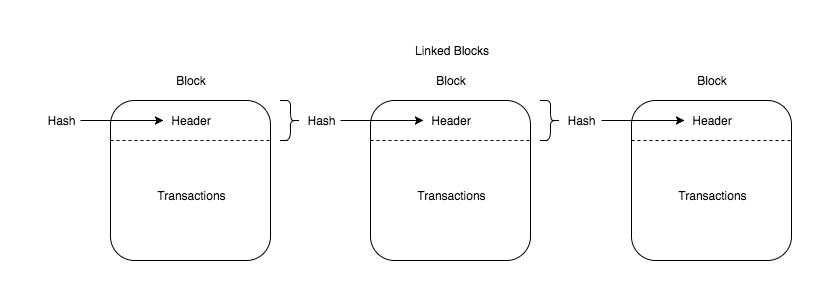
\includegraphics[scale=0.5]{img/blockchain}}
\caption{Schema semplificato di una blockchain}
\label{f:grids:arch}
\end{figure}

\subsection{Proof of Work}
\label{c:tec:bitcoin:pow}
L'algoritmo PoW consiste nel cercare un valore il cui hash (calcolato per esempio con SHA-256), quando viene calcolato, comincia con un certo numero di bit a zero. Il lavoro medio richiesto per trovare questa soluzione cresce in modo esponenziale al numero di bit nulli richiesti nell'hash e può essere verificato in modo estremamente semplice, ossia facendo l'hash del blocco.
Nel caso della rete Bitcoin, ogni blocco contiene un \textit{nonce} che viene incrementato finché il valore dell'hash non è quello desiderato. Questo processo richiede un certo \textit{lavoro} da parte della CPU appartenente al nodo "vincitore", e il blocco non può essere cambiato senza fare nuovamente il lavoro. In più, quando vengono accodati nuovi blocchi, il lavoro per modificarlo include anche il lavoro per modificare tutti gli altri blocchi che lo seguono. La caratteristica chiave che rende la blockchain immutabile è il fatto che, al variare anche solo di un singolo bit di un blocco, il suo hash cambia completamente, e quindi non contiene più il numero di bit più significativi a zero richiesti dal PoW. 
L'algoritmo risolve anche la questione di determinare la rappresentazione dei voti: se si basasse sul principio one-IP-address-one-vote, potrebbe essere facilmente sovvertito da qualsiasi attaccante che allocasse tanti indirizzi IP - questo attacco è conosciuto in letteratura come \textit{Sibyl Attack}, spiegato più avanti nel paragrafo \ref{c:integr:lib:bitcoinj}. La Blockchain si basa, invece, sul principio one-CPU-one-vote: la decisione adottata dalla maggioranza è rappresentata dalla catena più lunga, alla quale è stato investito il maggior sforzo computazionale. Se la maggioranza della potenza delle CPU della rete è controllata da nodi \textit{trusted}, la catena "onesta" sarebbe quella a crescere più velocemente e a superare tutte le altre; per modificare la blockchain, inoltre, un attaccante dovrebbe rieseguire il PoW del blocco che vuole modificare e di tutti quelli che lo seguono, e quindi dovrebbe equagliare e sorpassare il lavoro di tutti i nodi \textit{trusted}, cosa impossibile da fare per una minoranza.

Per compensare l'incremento della velocità dell'hardware, la difficoltà del PoW viene determinata da una media mobile del numero di blocchi creati all'ora: se vengono generati troppo velocemente, la difficoltà aumenta, in modo tale da mantenere la velocità a un blocco ogni circa 10 minuti. 
C'è una probabilità molto bassa che vengano generati più blocchi contemporaneamente, ma se dovesse accadere la blockchain, invece di "dividersi" come ci si aspetterebbe, si stabilizza velocemente.

I nodi che donano la loro capacità computazionale per risolvere il \textit{puzzle} e di fatto costruire la blockchain vengono chiamati \textit{miners}, e vengono premiati ogni volta che risolvono un blocco.


\subsection{Altri algoritmi di consenso: Proof of Stake}
\label{c:tec:bitcoin:pow}

Sono stati trattati in letteratura, oltre al PoW, altri algoritmi di consenso distribuito adatti all'utilizzo nella blockchain: uno di questi è il \textit{Proof of stake} (PoS)\cite{Li2005}. Nelle criptovalute PoS-based, come PeerCoin, il creatore del blocco successivo viene scelto in base a varie combinazioni tra selezione random, ricchezza o età (da qui la parola \textit{stake}, partecipazione).

Ci sono diverse tecniche di selezione del blocco, tra cui:

\begin{itemize}
    \item \textit{Randomized block selection}: Nxt e BlackCoin utilizzano la randomizzazione per designare il miner successivo, attraverso l'uso di una formula che va a vedere il valore di hash più piccolo insieme alla misura dello stake. Dal momento che questi ultimi sono pubblici, ogni nodo può predirre con ragionevole precisione quale nodo vincerà il diritto di estrarre un blocco.
    \item \textit{Coin age-based selection}: è il caso di Peercoin, il cui sistema combina la randomizzazione con il concetto di \textit{coin age}, un numero derivato dal prodotto del numero di monete per il numero di giorni in cui il denaro è stato mantenuto. Ciò vuol dire che insiemi di monete grandi e "vecchi" possono competere per generare il blocco successivo, però l'età viene azzerata non appena viene firmato un blocco e quindi il proprietario di quelle monete deve ricominciare da capo; inoltre, la probabilità di trovare il blocco successivo raggiunge il massimo valore dopo 90 giorni, in modo da evitare che si formino insiemi troppo "vecchi" di stake che dominerebbero la blockchain. Questo processo rende sicura la rete e produce gradualmente nuove cripto-monete col passare del tempo, senza consumare eccessive quantità di potenza computazionale. 
    \item \textit{Delegated Proof of stake} (DPoS): i sistemi che utilizzano questa modalità utilizzano un numero limitato di nodi per proporre e validare i blocchi. Ciò serve a mantenere i tempi di processamento delle transazioni bassi. EOS, ad esempio, utilizza soltanto 21 miners, la cui reputazione può aumentare o diminuire, consentendo ad altri nodi di sostituirli. 
    \item \textit{Randomized Proof-of-Stake} (RPoS): simile al DPoS, ma viene selezionata una "commissione" piuttosto che un nodo singolo. Ogni nodo viene scelto casualmente utilizzando un \textit{beacon} verificabile per proporre il blocco corrente di transazioni, e poi quest'ultimo viene verificato attraverso quel comitato di nodi.
\end{itemize}

\newpage

%%%%%%%%%%%%%%%%%%%%%%%%%%%%%%%%%%%%%%%%%%%%%%%%%%%%%%%%%%%%%%%%%%%%%%%%%%%%%%%%%%%%%%%

\chapter{GRIDS System}
\label{c:grids}
Il \textit{GRIDS System} (\textit{Generic Resilient Identity Services}) è un framework che sfrutta il paradigma Social Internet of Things (SIoT) per migliorare le operazioni di mapping ID-to-locator, in cui viene disaccoppiato l'host identifier (ID), assegnato univocamente a un oggetto, dal suo locator, cioè l'indirizzo fisico usato a livello di rete per il routing. Di conseguenza, è necessaria una funzione di mapping per tradurre l'ID del nodo di destinazione nel suo locator corrente (per esempio, il suo indirizzo IP): per fare ciò serve un'infrastruttura di mapping distribuita che si basa, per esempio, sulle \textit{Distributed Hash Tables} (DHT) e implica un costo e soprattutto un ritardo addizionale. La richiesta potrebbe attraversare più server prima che arrivi a quello che possiede l'informazione richiesta. L'idea proposta nel GRIDS System è quella di togliere il carico dall'infrastruttura di mapping navigando il grafo SIoT creato dalle relazioni che si stabiliscono tra gli oggetti.

\section{Architettura}
\label{c:grids:arch}

Nella figura \ref{f:grids:arch} è rappresentato uno schema dell'architettura del GRIDS System, in cui ogni nodo GRIDS fornisce un \textit{Relationship Service} (RS), in cui gli elementi sono spiegati più avanti.

\begin{figure}[h!t]
\centerline{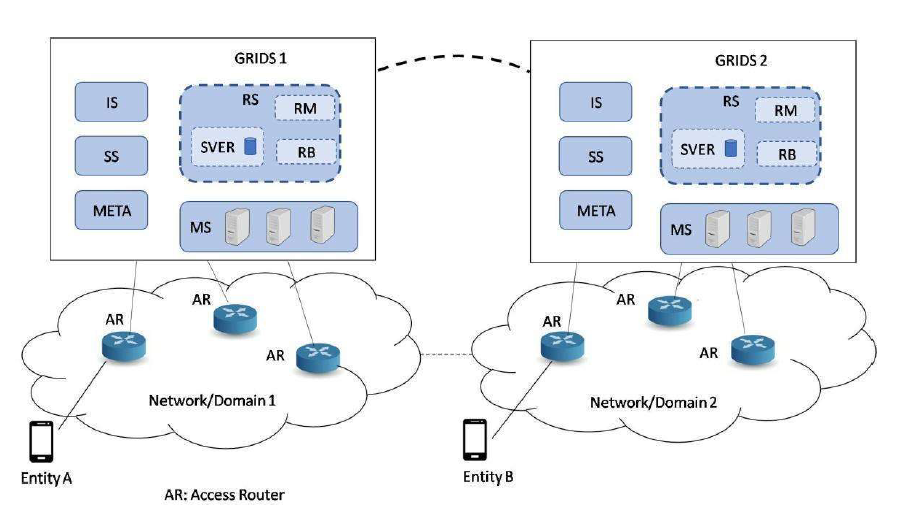
\includegraphics[scale=0.5]{img/GRIDSarch}}
\caption{Architettura del GRIDS System}
\label{f:grids:arch}
\end{figure}

In ogni RS si trova un RM (\textit{Relationship Manager}), un RB (\textit{Relationship Browser}) e uno SVER (\textit{Social Virtual Entity Repository}), i quali sono in run nello stesso server e condividono lo stesso locator nella rete.
I tipi di relazioni che vengono considerate nel sistema sono i seguenti:
\begin{itemize}
    \item \textit{Ownership Object Relationship} (\textbf{OOR}), creata tra oggetti che appartengono allo stesso proprietario;
    \item \textit{Co-location Object Relationship} (\textbf{CLOR}), creata tra dispositivi immobili che si trovano nello stesso luogo. Viene chiamata anche co-geolocation (CGLOR);
    \item Parental Object Relationship (\textbf{POR}), creata tra oggetti con stesso modello, produttore e lotto di produzione;
    \item \textit{Co-work Object Relationship} (\textbf{CWOR}), creata tra oggetti che si "incontrano" tra loro nel posto di lavoro del proprietario, come ad esempio il PC portatile e la stampante in un ufficio;
    \item \textit{Social Object Relationship} (\textbf{SOR}), creata come conseguenza di incontri frequenti tra oggetti, come succede tra smartphone che appartengono a persone che utilizzano lo stesso mezzo di trasporto pubblico ogni giorno per andare a lavoro/scuola, o persone che frequentano lo stesso bar/palestra/ristorante;
    \item \textit{Untrusted Object Relationship} (\textbf{UOR}), si riferisce a relazioni per dispositivi appena aggiunti per avere accesso alla rete sociale, come succede per esempio durante la connessione a uno stesso AP, oppure con i dispositivi nello stesso SVER;
    \item \textit{Transactional Object Relationship} (\textbf{TOR}), si origina quando due o più risorse interagiscono tra loro, come due persone che hanno una chiamata VoIP, una persona che ha accesso alle informazioni fornite da un sensore, due web service che si scambiano servizi, ecc.
\end{itemize}

\subsection{Relationship Manager}
\label{c:grids:rm}

La relazione tra due entità (e quindi tra le rispettive SVE) viene stabilita in modalità diverse, a seconda del tipo di relazione in questione. Alcune di esse (per esempio la OOR oppure la POR) sono legate al profilo della SVE, mentre altre dipendono dal comportamento dei dispositivi stessi (per esempio la SOR o la CLOR). Tutte queste informazioni vengono trasmesse tramite tag e metadata al RM, il quale deve processarle per stabilire le azioni di management da fare. 

\begin{figure}[h!t]
\centering
\subfloat[Elementi del RM]{
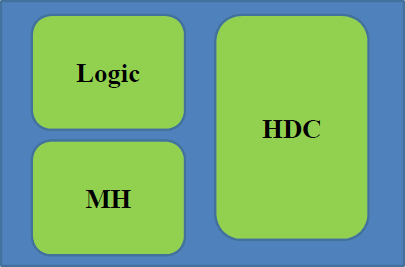
\includegraphics[height=100pt]{img/rma}
\label{f:grids:rma}}
\qquad % togliere se voglio far lievitare le pagine 
\subfloat[Componenti della logica del RM]{
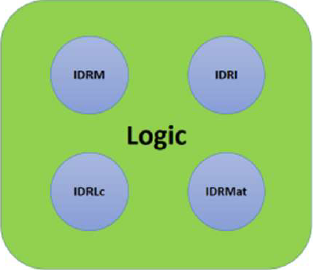
\includegraphics[height=100pt]{img/rmb}
\label{f:grids:rmb}}
\caption{Relationship Manager}
\label{f:grids:rm}
\end{figure}

Il RM è costituito da tre parti, come raffigurato nella figura \ref{f:grids:rma}. Gli algoritmi decisionali e i classificatori sono implementati nel modulo Logic, attraverso l'analisi dei tags e dei metadata delle SVE. Le informazioni utili per identificare le relazioni sono conservate temporaneamente nella \textit{Historical Data Cache} (HDC). Il \textit{Message Handler} (MH), infine, inoltra l'informazione sulle nuove relazioni ad altri RM affinch\'e le friendiship table delle SVE siano aggiornate, nel caso in cui le due SVE sono gestite da due diversi RM. Il MH, inoltre, pubblica i metadata e i tag dei \textit{monitored events}, i quali possono innescare la creazione/cancellazione di una nuova relazione e iscriversi all'evento stesso.

Gli elementi principali che compongono la logica del RM sono i seguenti (figura \ref{f:grids:rmb}):

\begin{itemize}
    \item \textit{ID Relation Initialization} (IDRI): inizializza le \textit{Friend Table} (FT) durante la registrazione di nuove entità, aggiungendo le prime relazioni (come OOR/POR/UOR) con le altre entità all'interno dello stesso SVER;
    \item \textit{ID Relation Management} (IDRM): implementa gli algoritmi e le procedure per stabilire, aggiornare ed eliminare le relazioni;
    \item \textit{ID Relation Lifecycle} (IDLc): valuta il lifecycle delle entittà gestite e fornisce statistiche rigurado le attività e i risultati dell'IDRM;
    \item \textit{ID Relation Maturity} (IDRMat): questo elemento interagisce con l'elemento incaricato di valutare l'affidabilità delle altre entità, per aggiornare di conseguenza i pesi delle relazioni.
\end{itemize}

\begin{figure}[h!t]
\centerline{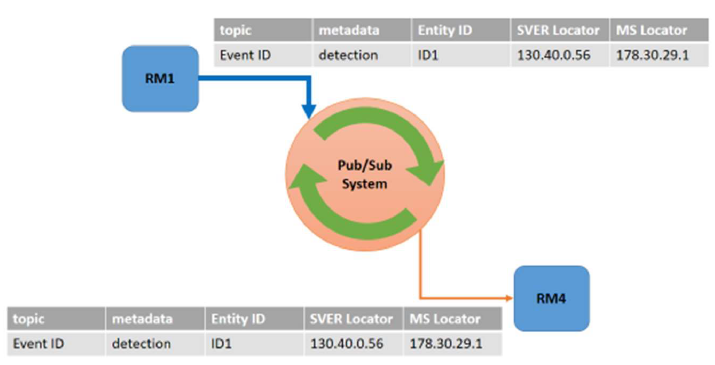
\includegraphics[scale=0.5]{img/scambiomessaggi}}
\caption{Propagazione degli eventi}
\label{f:grids:scambiomex}
\end{figure}

Le funzioni di \textit{relationship management} si affidano su due procedure di message-forwarding, che sono le seguenti:
\begin{itemize}
    \item \textit{New friendship alert}: generato e ricevuto quando viene stabilita un'amicizia tra due SVE che risiedono in diversi RM. Di conseguenza, un RM invia all'altro informazioni come: Entity ID, metadati, tipo di relazione, SVE locator e il locator del GRIDS-MS locator dell'amico che deve essere aggiunto nella FT della SVE di destinazione;
    \item \textit{Event alert}: trasmette informazioni circa alcuni eventi relativi a una SVE e che potrebbe causare la creazione di una nuova relazione. Queste informazioni devono essere valutate dai RM delle entità coinvolte (o dal singolo RM se le SVE risiedono nello stesso RM). Visto che non sempre sono noti i RM interessati a certi eventi, questa informazione dovrebbe essere diffusa a tutti i RM potenzialmente interessati. per fare ciò si utilizza il Pub/Sub System (PSS), come mostrato nella figura \ref{f:grids:scambiomex}. L'EventID in figura identifica l'argomento di interesse, per esempio: EventID=“AP address A677.7BCD.F345”. Questa informazione viene diffusa cosicch\'e gli altri RM sanno che quell'entità ricade sotto la copertura dell'AP con MAC address A677.7BCD.F345.
\end{itemize}

\section{Implementazione}
\label{c:grids:implementation}

L'implementazione del GRIDS System è stata realizzata nel linguaggio Java. Nello specifico, è stato utilizzato Java Enterprise Edition per creare una Web Application, la quale è stata deployata su un Application Server: nel nostro caso si tratta di Glassfish 5.0.0, che è pensato appositamente per le implementazioni della Java Platform.

Il sistema è distribuito su più macchine, le quali comunicano tramite RMI\footnote{https://docs.oracle.com/javase/tutorial/rmi/index.html} (\textit{Remote Method Invocation}), una tecnologia il cui scopo è quello di rendere trasparenti al programmatore i dettagli della comunicazione in rete. I nodi prendono il nome di Server, e sono interconnessi tra loro per formare una rete peer-to-peer. Ognuno di essi viene identificato dal Server ID.

La classe in cui vengono definiti i metodi remoti è \textit{GridsSystem}, che implementa l'interfaccia root RMI. Nel listing \ref{gridssys} è riportata la struttura del codice di questa classe.

La classe \textit{CustomSimulation} contiene il metodo initNetwork() per inizializzare il Server: viene creata un'istanza di GridsSystems e viene effettuato il lookup dell'interfaccia RMI remota per la registrazione del server, richiamando il metodo remoto della classe GridsSystem. Il tutto viene avviato tramite la GUI contenuta nella classe \textit{EngineSimulator}, mostrata nel paragrafo successivo in figura \ref{f:grids:gui1}.
Sempre nella funzione initNetwork() vengono instaurate le relazioni tra i nodi, in pieno accordo con il paradigma Social IoT. I parametri utilizzati nella creazione delle relazioni sono le coordinate geografiche dei nodi (che si ottengono dalle informazioni contenute nelle piattaforme IoT che "ospitano" i nodi) e le probabilità di creazione delle relazioni (fornite attraverso il file di configurazione \textit{probabilities.ini}). Per esigenze di testing, i tipi di relazioni (come ad esempio OOR, SOR, CLOR) sono assegnati casualmente.

\begin{lstlisting}[caption={GridsSystem.java},label={gridssys},style={c}]

public class GridsSystems extends UnicastRemoteObject implements RMIRootInterface {

    HashMap<String, String> servers_address;

    public GridsSystems() throws RemoteException {
        super();
        servers_address = new HashMap<>();
    }

    @Override
    public void RegisterServer_address(String address, String id) {
        this.servers_address.put(address, id);
        System.out.println("SERVER REGISTERED: " + "//" + address + "/server" + id + "\n");
    }
\end{lstlisting}

Oltre queste, è disponibile una risorsa REST per poter consultare i dati non solo del Server corrente, ma anche degli altri Server attivi nel sistema. Le chiamare HTTP disponibili sono le seguenti:

\begin{itemize}
    \item GET all'indirizzo "/Sim/SIoT/Server/{id}/SVER/{uid}" per ricevere la lista delle relazioni del nodo \textit{uid} contenuto nello SVER del server \textit{id};
    \item GET a "/Sim/SIoT/Server/{id}/{uid}" per ottenere le proprietà della singola SVE (id e uid come la richiesta sopracitata);
    \item GET a "/Sim/SIoT/Server/{id}/Clients" per ottenere l'elenco dei Client contenuti nel server {id};
    \item GET al path "/Sim/SIoT/Server/0/Entities" per BOH. 
    
\end{itemize}

Ciò è possibile grazie alla presenza del database MySQL con cui il sistema interagisce attraverso la classe \textit{GridsRS}, ossia il Relationship Manager della specifica, e alla classe \textit{Server}. Quest'ultima implementa un'ulteriore interfaccia RMI, riportata qui di seguito nel listing \ref{rmiInterface}.




\begin{lstlisting}[caption={RMIInterface.java},label={rmiInterface},style={c}]

public interface RMIInterface extends Remote {

    public RelBrowser getRelBrowser() throws RemoteException;
    public HashSet<HashMap> getGRIDS_MS() throws RemoteException;
    public void addMap_GRIDS(HashMap map) throws RemoteException;
    public HashMap<ClientInterface, Sve> getGRIDS_RS() throws RemoteException;
    public void updateGRIDS_RS(ClientInterface c, Sve sve) throws RemoteException;
    public void fillGRIDS_RS() throws RemoteException;
}
\end{lstlisting}

La classe \textit{Server} contiene anche gli attributi che caratterizzano il nodo stesso, i quali sono: l'ID, l'indirizzo IP, il GridsRS, il GridsMS (\textit{GRIDS Mapping Service}), che di fatto realizza la corrispondenza tra ID del nodo e indirizzo IP corrispondente, e il \textit{RelBrowser}, che è l'oggetto responsabile della navigazione nel grafo delle relazioni sociali tra i nodi.
Oltre al \textit{RelBrowser}, altre classi utili per la navigazione delle relazioni sociali sono \textit{FriendTableEntry} e \textit{SVE}, che saranno descritte più avanti.

Per poter accedere ai dati predenti nei canali Thingspeak o alle risorse di FESTIVAL sono disponibili delle librerie apposite.

Per quanto riguarda il livello di \textit{Data Access}, essa è composta da due database: \textit{social\_iot\_platform} e \textit{social\_iot\_platform\_sve}. Il primo contiene la tabella denominata sver, la quale contiene l'elenco dei Client che fanno riferimento allo stesso SVER, che di fatto è il Server che contiene la tabella stessa. Le colonne sono composte dai seguenti campi:

\begin{itemize}
    \item \textbf{channel}: codice che identifica, nel caso in cui il nodo sia virtualizzato da Thingspeak, il canale della piattaforma:
    \item \textbf{uid}: ID del client;
    \item areas: coordinate geografiche nelle quali è posizionato il nodo;
    \item \textbf{ip}: sempre nel caso si tratti di Thingspeak, è l'indirizzo web del nodo (ad esempio: https://thingspeak.com/channels/156761);
    \item \textbf{meta}: eventuali metadati (ad esempio una descrizione del nodo);
    \item \textbf{server}: ID del server che contiene la SVE;
\end{itemize}

Il database \textit{social\_iot\_platform\_sve}, invece, contiene un numero di tabelle pari al numero di Client nello SVER, all'interno delle quali si trova l'elenco degli amici della SVE. Le colonne di ogni tabella sono:

\begin{itemize}
    \item \textbf{ifFriend}: uid della SVE con cui è definita la relazione;
    \item \textbf{REL}: tipo di relazione costituita;
    \item \textbf{MS\_LOCATOR}: indirizzo IP del Server che fa da GridsMS per il nodo "amico"; 
    \item \textbf{SVE\_LOCATOR}: indirizzo IP in cui si trova la SVE 
    \item \textbf{Server}: ID del Server in cui si trova la SVE dell'"amico".
\end{itemize}

Le classi necessarie per realizzare il mapping con il database sono le seguenti: 
\begin{itemize}
    \item la classe \textit{Client}, che mappa le SVE, in particolare i record della tabella sver;
    \item la classe \textit{FriendTableEntry}, che rappresenta il singolo record contenuto nelle tabelle del database social\_iot\_platform\_sve;
    \item \textit{SVE}, lista di FriendTableEntry.
\end{itemize}

Notare che, anche se contengono dati diversi, le classi Client e SVE rappresentano lo stesso concetto: la virtualizzazione del nodo IoT visto sia come entità sociale, sia come semplice dispositivo.

Il driver utilizzato per l'interazione tra il codice Java e il database MySQL è JDBC\footnote{https://www.oracle.com/technetwork/java/javase/jdbc/index.html} (\textit{Java Database Connectivity}), che fornisce una serie di API per effettuare query e per aggiornare dati in un database, ed è orientato per database relazionali.

In figura \ref{f:grids:diagramma} è possibile osservare il diagramma delle classi principali dell'architettura del Grids System. Notare che sono raffigurate soltanto le classi, i metodi e gli attributi necessari per la descrizione del sistema: le classi delle librerie di Thingspeak e FESTIVAL, per esempio, sono state omesse per semplicità.


\begin{figure}[h!t]
\centerline{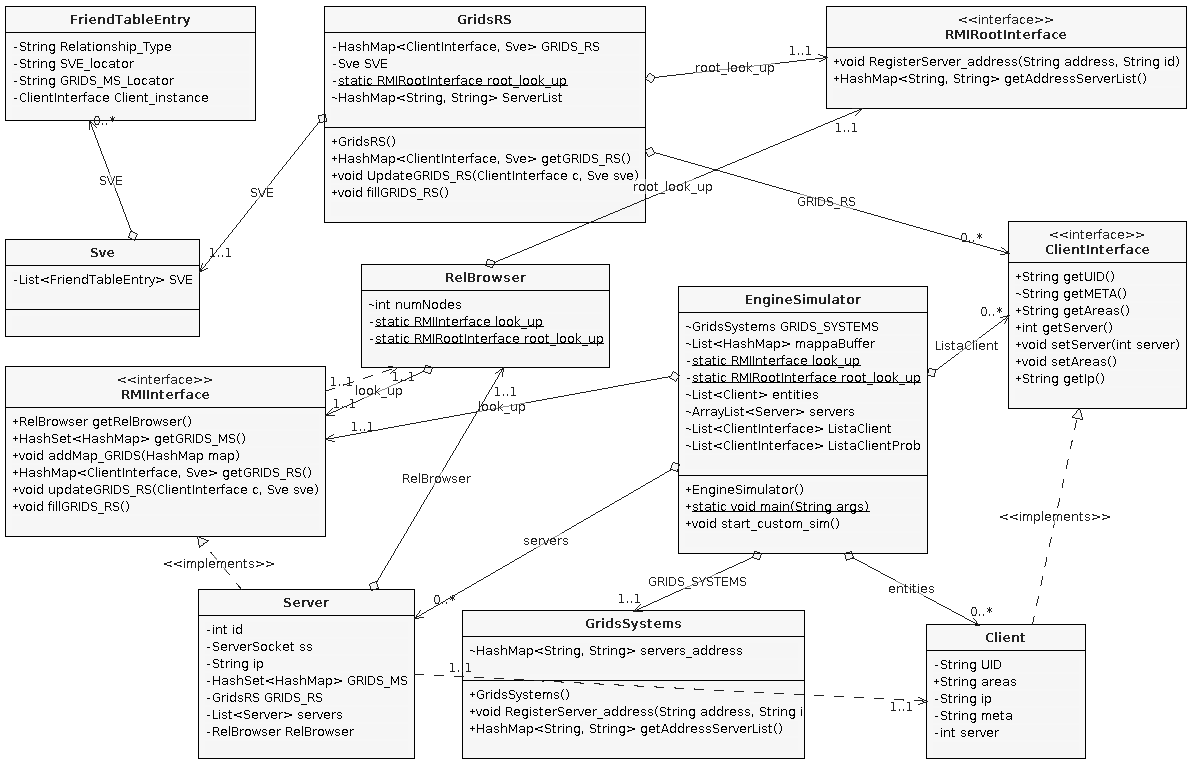
\includegraphics[width=\textwidth]{img/initialDiagramCorrect}}
\caption{Diagramma delle classi del Grids System}
\label{f:grids:diagramma}
\end{figure}


\section{Caso d'uso d'esempio}
\label{c:grids:usecase}

Per effettuare il deployment della piattaforma è necessario aprire il progetto Java con un IDE, in questo caso Netbeans IDE 8.2. Bisogna inoltre assicurarsi che il database sia in run: è possibile utilizzare XAMPP per Linux 5.6.20, che permette di avviare velocemente non solo MySQL, ma anche server Apache e i linguaggi di programmazione PHP e Perl, utili per lo sviluppo di semplici applicazioni Web (nonostante ciò, questi ultimi non sono necessari per l'avvio del Grids System). 

Fatto ciò, bisogna settare correttamente gli indirizzi IP di Server, Gateway e SVER e l'ID del server. Nel caso d'uso base, visto che il Server avviato è solo uno, l'ID è pari a 0. 

\begin{figure}[h!t]
\centerline{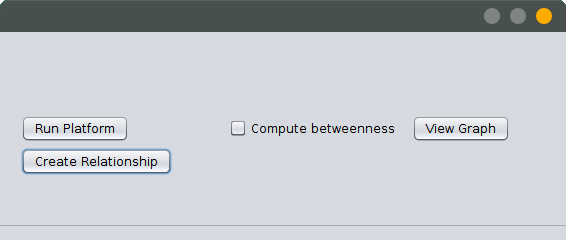
\includegraphics[scale=2.5]{img/gui1}}
\caption{GUI del Grids System}
\label{f:grids:gui1}
\end{figure}

Poi bisogna avviare il progetto, il quale verrà deployato sul Glassfish server, e l'interfaccia grafica, raffigurata in figura \ref{f:grids:gui1}.
Per avviare la piattaforma, bisogna cliccare sugli appositi jButton \textit{Run Platform} e \textit{Create Relationship}, rispettivamente per effettuare la configurazione RMI e per creare le relazioni tra le Social Virtual Entities. Infine, cliccando sul tasto \textit{View Graph} è possibile visualizzare il grafo delle relazioni, come raffigurato in figura \ref{f:grids:gui2}. È possibile selezionare i singoli nodi del grafo per visualizzare un'ulteriore finestra in cui sono contenute le informazioni della SVE corrispondente.

\begin{figure}[h!t]
\centerline{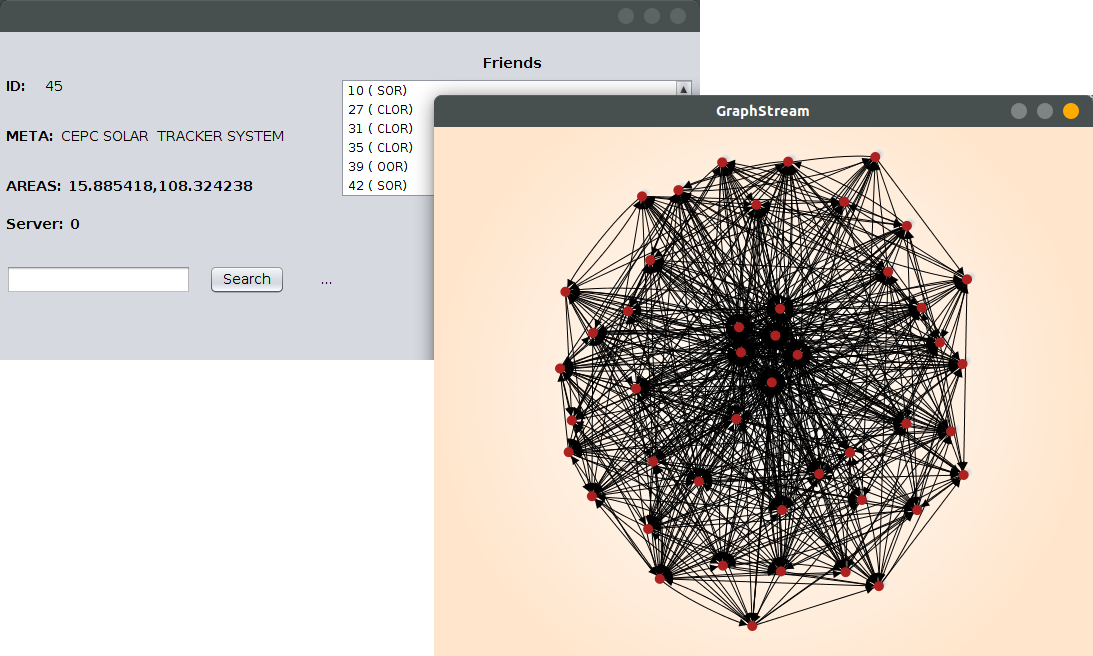
\includegraphics[width=\textwidth]{img/gui2}}
\caption{Grafo delle relazioni SIoT}
\label{f:grids:gui2}
\end{figure}

Nel capitolo successivo, la struttura appena presentata verrà ampliata e arricchita per contenere un wallet Bitcoin, e quindi la possibilità di ricevere denaro dagli utenti che si connetteranno alla rete SIoT e di inviarlo ai proprietari di dispositivi smart che espongono tramite questa piattaforma.
\newpage

%%%%%%%%%%%%%%%%%%%%%%%%%%%%%%%%%%%%%%%%%%%%%%%%%%%%%%%%%%%%%%%%%%%%%%%%%%%%%%%%%%%%%%%

\chapter{Integrazione del GRIDS System con la Blockchain}
\label{c:integr}
\section{Modello teorico}
\label{c:integr:model}

Prima di cominciare lo sviluppo, è di vitale importanza pensare al modello di integrazione della blockchain nel sistema, rappresentato in figura \ref{f:integr:modello}. 

%% METTERE IMMAGINE DEL MODELLO FINALE
% per l'immagine si fa una nuvoletta che rappresenta la siot, con dei cerchi che rappresentano i Server. i final client si connettono ai Server e le piattaforme 

Verrà creata un'applicazione che sarà utilizzata dall'utente finale per comprare i dati dei nodi della rete. 
Ognuna di esse è in grado di effettuare le transazioni, che saranno poi incluse nella blockchain. Ogni utente, attraverso l'applicazione, si connette con un nodo Server del GRIDS System. Quest'ultimo è incaricato di prendere i dati delle SVE che ospita (il Server stesso o gli altri Server della rete SIoT), attraverso i meccanismi di discovery descritti nel capitolo \ref{c:grids}, e di restituire i risultati all'utente finale. 

I proprietari dei nodi virtualizzati ed esposti attraverso la rete SIoT riceveranno il denaro virtuale, ma il GRIDS System terrà per sè una piccola percentuale del prezzo presentato all'utente finale.

I dati che verranno scambiati sono: l'utente fornisce ID del nodo a cui è interessato, il server risponderà con il prezzo dei dati corrispondenti. L'utente, venuto a conoscenza del prezzo, effettuerà la transazione e riceverà in cambio i dati del nodo IoT, oppure, nel caso si tratti di un nodo che appartiene a un canale Thingspeak, la readAPIkey con la quale l'utente potrà andare a leggere i dati autonomamente attraverso la piattaforma.

In sostanza, non vengono acquistati i dati direttamente dal sensore, ma viene aggiunto un livello di indirezione tra utente e nodo IoT, mantenendo il sistema ugualmente distribuito e decentrato, grazie all'utilizzo della blockchain.

I casi d'uso con cui verrà effettuato il testing riguarderanno un nodo Server del GRIDS System e un Client, ma sarà possibile utilizzare il sistema con una rete di Server e con Client multipli.

Sarà sviluppato, inoltre, un meccanismo di "ricarica" che permetterà al sistema di aggirare i tempi di conferma delle transazioni, che come sappiamo sono una caratteristica imprescindibile di qualsiasi blockchain, con il quale i client potranno effettuare un'unica transazione più grande e successivamente attingere dal credito residuo ogni qual volta desiderano acquisire dati dal sistema.

\section{Scelta della Blockchain}
\label{c:integr:lib}

La prima cosa da considerare per lo sviluppo del sistema è in modo in cui la blockchain può essere integrata. Sono possibili due principali modalità:
\begin{itemize}
    \item implementazione \textit{from scratch};
    \item utilizzo di una blockchain esistente.
\end{itemize}

L'implementazione \textit{from scratch} è una scelta poco pratica poiché è molto difficile reperire le risorse necessarie per il deployment di una blockchain, come ad esempio un numero considerevole di calcolatori per formare la rete di miners, e potenza computazionale sufficiente per l'esecuzione di un algoritmo per il raggiungimento del consenso.

Quindi la scelta naturale è l'uso di una blockchain preesistente attraverso \textit{reference implementation} o librerie. Nello specifico, è stata scelta la rete Bitcoin, con una community molto estesa di developer e un set di tool per potervi interagire, tra cui Bitcoinj\footnote{https://bitcoinj.github.io/}, una libreria implementata in Java, stesso linguaggio di programmazione utilizzato per lo sviluppo del GRIDS System. Le caratteristiche di questa libreria sono illustrate nel paragrafo \ref{c:integr:lib:bitcoinj}.
Un'altra feature della rete Bitcoin che ha influito positivamente sulla scelta della blockchain è la presenza di una Testnet, cioè una rete separata da Bitcoin Core in cui le transazioni non hanno alcun valore monetario. Essa è approfondita nel paragrafo \ref{c:integr:lib:testnet}.


\subsection{Bitcoinj}
\label{c:integr:lib:bitcoinj}

Bitcoinj è una libreria per lavorare con il protocollo Bitcoin. Può mantenere un wallet, inviare/ricevere transazioni senza aver bisogno di una copia locale di Bitcoin Core e ha molte altre caratteristiche avanzate. È implementata in Java, ma può essere utilizzato da qualunque linguaggio di programmazione JVM-compatible (come JavaScript).

Una caratteristica peculiare di Bitcoinj è la presenza della \textit{Simplified Payment Verification} (SPV): in questa modalità viene scaricata solo una piccola parte della blockchain, quindi è possibile utilizzare la libreria in dispositivi constrained, come i nodi dell'IoT. 

Altre caratteristiche di Bitcoinj sono: 
\begin{itemize}
    \item una \textit{wallet class} con cifratura, calcolo delle \textit{fees} (commissioni), derivazione deterministica della chiave e event listener che permettono di tenere aggiornato il saldo del wallet;
    \item un'applicazione con GUI per il wallet da utilizzare come base per le proprie app;
    \item \textit{full verification mode} sperimentale, che svolge lo stesso processo di verifica di Bitcoin Core. In questa modalità, il set di \textit{unspent transaction output} (UTXO set) viene calcolato e indicizzato in un database, permettendo un lookup veloce del saldo del wallet;
\end{itemize}

Ora andiamo ad approfondire il modello di sicurezza di Bitcoinj. Come gi\`a detto, questa libreria supporta due modalità: \textit{full verification} e \textit{simplified verification}. Esse controllano l'uso delle risorse dell'applicazione e quanta fiducia viene riposta negli altri partecipanti nel sistema Bitcoin. 

Come illustrato nel paragrafo \ref{c:tec:blockchain:funzionamento}, un nodo full mantiene un database di unspent outputs, e le transazioni che cercano di spendere output che non esistono oppure sono già stati spesi vengono ignorate. I blocchi vengono risolti dai miners e vengono inviati in broadcast nella rete cosicché tutti possano essere d'accordo sull'ordine delle transazioni e nodi che non vedono il broadcast di una certa transazione (per esempio perché erano offline in quel momento) possano recuperarla. 
Le operazioni di controllo, store e aggiornamento del database per ogni singola transazione è molto intenso; anche recuperare lo stato corrente del database from scratch è un'operazione molto lenta. Per questa ragione, non tutti i dispositivi possono mantenere un full node.

Con la SPV, invece, vengono memorizzate solo le transazioni rilevanti per il wallet in questione, mentre le altre vengono cancellate o direttamente mai scaricate. Le transazioni broadcast vengono sempre ricevute, però non ne viene controllata la validità. Questa modalità operativa è veloce e leggera abbastanza da essere eseguita su uno smartphone, ma può essere soggetta ad attacchi potenziali, illustrati qui di seguito: 

\begin{enumerate}
    \item \textit{Sybil attack}: consiste nel dirottare l'intera connessione internet della vittima e connetterla a una rete farlocca. È più facile da portare a termine quando viene utilizzata una connessione internet untrusted, come ad esempio reti Wi-Fi pubbliche, oppure utilizzando Tor. Bitcoinj non supporta Tor, quindi gli interessati da questo attacco possono essere i wallet mobili; 
    \item \textit{Finney attack}: consiste nel risolvere un blocco che contiene un double spend, comprare un servizio, e poi inviare in broadcast il blocco.
\end{enumerate}

Per spiegare meglio il funzionamento di questi attacchi, bisogna prima introdurre il concetto di \textit{pending transaction}.

Una \textit{pending transaction} è una transazione non ancora inclusa nella blockchain; in altre parole, è lo stato che assume non appena viene diffusa nella rete. I nodi miners che vedono questa transazione, ne controllano la validità e, se il risultato è positivo, la includono nel blocco che al momento stanno provando a risolvere. Naturalmente, quelle non valide vengono ignorate.

L'applicazione del client riceverà le \textit{pending transactions}, le aggiungerà al wallet e avvierà gli event listener. Tuttavia, nella modalità SPV l'unico motivo che si ha per credere che la transazione sia valida è il fatto che i nodi a cui si è connessi trasmettano la transazione nella rete. Se un'applicazione fosse connessa a un nodo malevolo, quest'ultimo potrebbe passare all'applicazione delle transazioni completamente invalide (come \textit{double spend} o addirittura transazioni con soldi inesistenti), e verrebbero ugualmente prese per buone. 

Dato che le applicazioni sviluppate con Bitcoinj non accettano connessioni in entrata, i peer con cui esse comunicano sono sempre scelti in maniera casuale all'avvio, quindi diventa estremamente difficile per un aggressore controllarne la connettività. Per questa ragione, il numero di peer che hanno confermato una transazione viene esposto attraverso l'oggetto \textit{TransactionConfidence}, e l'applicazione è in grado di monitorarlo per avere questo tipo di informazione. Questa feature, come verrà spiegato più avanti, sarà molto utile per lo sviluppo dei wallet del GRIDS System.

Una volta che la maggior parte dei peer hanno confermato quella transazione, si può essere abbastanza sicuri che essa si sta propagando attraverso la rete e con ogni probabilità è valida: ecco il motivo principale per cui il Sybil attack è molto improbabile.

In un Finney attack, invece, l'attaccante crea un blocco che include una transazione tra due indirizzi controllati da lui. Una volta estratto il blocco, non lo diffonde subito, ma invece va a spendere quella valuta da qualche venditore che accetta transazioni non confermate. Una volta ottenuti i beni dal venditore, diffonde il blocco contenente il double spend, e quindi riceve i soldi indietro. Tutto questo processo richiede una buona dose di tempismo e pazienza da parte dell'attaccante: non solo deve risolvere correttamente il blocco, ma deve anche effettuare velocemente l'acquisto del bene, prima che un altro miner riesca a risolvere e a diffondere un altro blocco valido. In conclusione, un utente che vende beni in maniera irreversibile, in maniera veloce e che accetta transazioni non confermate è suscettibile a un attacco Finney.

Questo problema viene risolto da parte di Bitcoinj attraverso l'utilizzo della \textit{Transaction Confidence}: se qualcuno perpetra un attacco, la confidence per quella transazione assumerà il valore \textit{DEAD}, il che significa che la transazione è come invertita e non verrà considerata per il conteggio del wallet della vittima.
La \textit{transaction confidence} è lo strumento di forza di Bitcoinj: permette di sapere se una certa transazione è inclusa o meno nella blockchain. 
Quando una transazione viene aggiunta nella blockchain, la transaction confidence assume il valore \textit{BUILDING} e si può accedere alla \textit{transaction depth}, ossia il numero di blocchi che sono stati costruiti a partire dal blocco della transazione stessa (per esempio, una transazione appena confermata ha depth uguale a 1).
Inoltre, sono implementati degli event listener che, ascoltando gli eventi della rete, possono essere usati per scatenare azioni specifiche nell'applicazione utente, come spedire beni o servizi soltanto quando viene raggiunto un certo livello di confidence.

Nel caso del nostro sistema, i listener che monitorano la confidence delle transazioni serviranno per innescare lo scambio di dati tra i client e la piattaforma SIoT.

%%%%%%%%%%%%%%%%%%%%%%%%%%

\subsection{Testnet}
\label{c:integr:lib:testnet}

La Testnet è un'alternativa alla blockchain della rete Bitcoin ufficiale, per essere utilizzata a fini di testing. Le monete della Testnet sono separate e distinte dai bitcoin reali e non hanno alcun valore. Ciò permette agli sviluppatori di applicazioni bitcoin-based di evitare di utilizzare veri bitcoin, senza la preoccupazione di perderli o di rompere la blockchain principale.

Per utilizzare la Testnet invece della rete principale, basta inserire un flag nell'applicazione: nel caso specifico di Bitcoinj, bisogna selezionare i \textit{Network Parameters} relativi alla Testnet.

La testnet è attualmente alla terza versione. La prima era stata superata poiché aveva il grosso problema secondo cui gli utenti cominciavano a scambiare la valuta della testnet con bitcoin reali, quindi è stata introdotta la versione 2, superata ulteriormente dalla versione attuale, che verifica le transazioni in minor tempo e contiene all'interno della propria blockchain transazioni \textit{edge-case} che ne testano la compatibilità implementativa.

Le differenze con la rete Bitcoin ufficiale sono:
\begin{itemize}
    \item il protocollo di rete della testnet utilizza la porta 8333 invece che la 18333 della rete Bitcoin;
    \item i valori nel campo ADDRESSVERSION sono differenti, per assicurare che nessun indirizzo della testnet funzioni nella rete Bitcoin;
    \item vi sono diversi header nel messaggio del protocollo: 0x0B110907 della rete ufficiale contro 0xF9BEB4D9 della testnet;
    \item la difficoltà minima di 1.0 nella testnet è uguale alla difficoltà 0.5 della rete principale. Ciò significa che la difficoltà della testnet è doppia rispetto a quella della rete Bitcoin. Inoltre, se nessun blocco viene risolto entro 20 minuti, la difficoltà viene resettata al valore minimo;
    \item un genesis block diverso;
    \item nella testnet è possibile utilizzare transazioni non-standard.
    \item la testnet riceve meno transazioni rispetto la blockchain principale ed è solitamente più piccola in termini di GB.
\end{itemize}

Per acquisire bitcoin utili per operare nella testnet, si possono utilizzare delle \textit{faucet} dalle quali è possibile ricevere valuta di testing\footnote{https://testnet.manu.backend.hamburg/faucet}. È buona norma, dopo averli utilizzati, ridare indietro i bitcoin alla faucet.

\section{Interfaccia Web e REST}
\label{c:integr:webrest}

È stata costruita un'interfaccia web con Angular 2 che interagisce con l'interfaccia REST del sistema, per rendere più agevole l'interazione con il sistema. In figura \ref{f:integr:gui-web} è rappresentata la GUI.

\begin{figure}[h!t]
\centerline{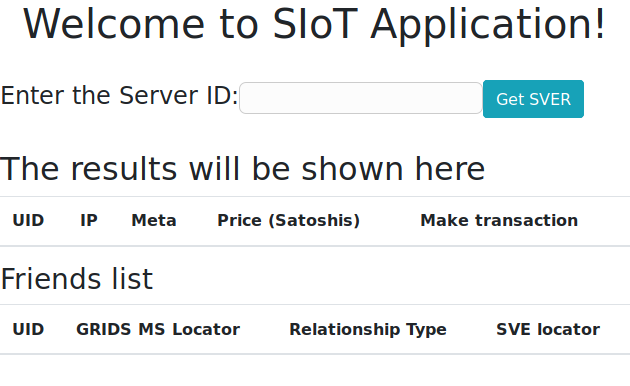
\includegraphics[scale=2.5]{img/gui-web-app}}
\caption{Interfaccia grafica della web app}
\label{f:integr:gui-web}
\end{figure}

Per quanto riguarda le REST API, invece, è stata aggiunta nella risorsa REST "Server" (a fini di testing) una richiesta che effettua una transazione da parte del server SIoT verso il wallet del proprietario del nodo IoT per ottenere alcuni dati, per esempio l'elenco delle relazioni del nodo.
\begin{itemize}
    \item Metodo: GET
    \item Path: "{id}/SVER/{uid}/Transaction/{amount}/{address}"
\end{itemize}

I parametri \textit{id} e \textit{uid} sono analoghi a quelli citati nel paragrafo \ref{c:grids:implementation}, mentre \textit{amount} e \textit{address} sono rispettivamente il numero di satoshi da inviare e l'indirizzo del wallet di destinazione.

È stata inoltre aggiunta la risorsa REST aggiuntiva "Transaction", di cui è riportato un estratto nel listing \ref{restResource}, che raccoglie le richieste per l'interazione con il Transaction Manager. È stata definita una richiesta che permette di visualizzare i dati ottenuti a seguito di una transazione.
\begin{itemize}
    \item Metodo: GET
    \item Path: "{trxHash}", dove trxHash è l'hash della transazione di cui si vuole visualizzare il risultato.
\end{itemize}

Nel caso d'uso considerato per lo sviluppo del sistema, con questa richiesta verrà restituita la \textit{Thingspeak readAPIkey} corrispondente al nodo di cui si desiderano i dati.


\begin{lstlisting}[caption={TransactionResource.java},label={restResource},style={c}]

@GET
@Path("{trxHash}")
@Produces(MediaType.TEXT_PLAIN)
public String visualizeData(@PathParam("trxHash") String trxHash) {
    // search the trx in the DB
    trxManager = new TrxManager();
    String result;
    if (trxManager.isUnconfirmed(trxHash)) {
        result = "Waiting for transaction validation...";
    } else {
        // get the data of transaction
        result = trxManager.getCompletedTrx(trxHash);
    }
    trxManager.closeConnection();
    return result;
}
\end{lstlisting}

\section{Database}
\label{c:integr:db}

Per quanto riguarda la parte di Data Access, è stato creato un nuovo database, oltre ai due preesistenti, chiamato \textit{social\_iot\_platform\_transaction}, in cui sono contenute quattro tabelle necessarie per l'implementazione delle transazioni.

La tabella "completed" contiene tutte le transazioni che sono state incluse nella Blockchain, insieme ai dati da restituire al Final Client. I campi sono i seguenti:

\begin{itemize}
    \item \textbf{TrxHash}: hash della transazione confermata;
	\item \textbf{content}: stringa con i dati.
\end{itemize}

La tabella "unconfirmed" contiene tutte le transazioni non ancora confermate. I campi sono:

\begin{itemize}
    \item \textbf{TrxHash}: hash della transazione da confermare;
    \item \textbf{SVER\_ID} e \textbf{SVE\_ID} del nodo di cui sono stati richiesti i dati.
\end{itemize}

La tabella "creditCharges" registra tutte le ricariche eseguite dagli utenti:

\begin{itemize}
    \item \textbf{trxHash}: hash della transazione confermata;
	\item \textbf{userID}: numero identificativo del Final Client. Al momento viene settato manualmente per ogni utente, ma successivamente potrebbe essere implementato un meccanismo di "log in" in cui sarà il GRIDS System a fornire dinamicamente un ID;
	\item \textbf{credit}: valore del credito ricaricato (in satoshi);
	\item \textbf{isConfirmed}: valore booleano che memorizza se la transazione è stata inclusa o meno nella Blockchain. Delle funzioni apposite del Transaction Client (paragrafo \ref{c:integr:trxmanager}) provvederanno a impostare il valore corretto di questo campo.
\end{itemize}

La tabella "readAPIkeys", infine, contiene, come dice il nome stesso, le readAPIkey di tutti i nodi ospitati dal GRIDS System. Essa verrà consultata 

\section{RMI registry}
\label{c:integr:rmi}

La Java API che permette di eseguire la \textit{remote method invocation} è l'elemento fondamentale della comunicazione tra le entità del sistema. Oltre all'interfaccia già esistente per l'interazione tra i Server del GRIDS System, è stata creata un'ulteriore interfaccia RMI per la comunicazione tra Server e Final Client: quest'ultima, però, è stata separata dalla prima per garantire il disaccoppiamento tra i metodi invocabili dai Server per la creazione dei propri wallet e i metodi per la richiesta di dati da parte dei Final Client. Perciò è presente un processo aggiuntivo in ascolto sulla porta 4849, diverso dal processo rmiregistry in ascolto sulla porta di default 1099, nella quale verrà effettuato il binding dei metodi della FinalClientRMIRootInterface, illustrata più avanti.

I metodi che sono stati aggiunti all'interfaccia RMI già esistente sono i seguenti:

\begin{itemize}
    \item CreateWallet(): permette la creazione del wallet destinato al nodo Server;
    \item getWalletBalance(): restituisce la quantità di valuta presente all'interno del wallet;
    \item makeTransaction(String destAddress, String amount): permette di effettuare una transazione di una quantità \textit{amount} di bitcoin all'indirizzo \textit{destAddress}.
\end{itemize}

I metodi dell'interfaccia FinalClientRMIRoot, riportati nel listing \ref{FinalClientRMIRootInterface}, vengono implementati all'interno del Server, e sono accessibili dai Final Client. Essi sono:

\begin{itemize}
    \item requestDataWithTrx(): aggiunge la transazione nella lista di quelle non confermate e restituisce l'indirizzo web in cui verranno visualizzati i risultati una volta che la transazione sarà validata;
    \item rechargeCredit(): ricarica il credito dell'utente con \textit{userID};
    \item getCredit(): restituisce il valore del credito residuo (in satoshi) dell'utente con \textit{userID};
    \item requestDatawithCredit(): permette di effettuare la richiesta dei dati 
\end{itemize}

\begin{lstlisting}[caption={FinalClientRMIRootInterface.java},label={FinalClientRMIRootInterface},style={c}]

public interface FinalClientRMIRootInterface extends Remote {
    
    public String requestDataWithTrx(String txHash, String SVER_ID, String SVE_ID) throws RemoteException;
    
    public String rechargeCredit(String trxHash, int userID, int amount) throws RemoteException;
    
    public int getCredit(int userID) throws RemoteException;
    
    public String requestDatawithCredit(String SVER_ID, String SVE_ID, int userID) throws RemoteException;
}

\end{lstlisting}

Nell'implementazione dei metodi appena elencati vengono istanziati oggetti di una classe chiamata \textit{Transaction Manager}, il punto focale del meccanismo di esecuzione e verifica delle transazioni, ma anche dell'accesso ai dati. Nel paragrafo \ref{c:integr:trxmanager} sarà illustrato nel dettaglio.

\section{Wallet Bitcoin e Transaction Manager ?}
\label{c:integr:trxmanager}


Il wallet Bitcoin, prima di essere integrato all'interno del GRIDS System, è stato sviluppato separatamente, come mostrato nel diagramma \ref{f:integr:trxclient}, ??per esigenze di testing??. L'interfaccia \textit{TransactionIf} contiene le \textit{signature} delle funzioni basilari per il funzionamento del wallet, come ad esempio makeTransaction(). La classe \textit{TransactionClient} contiene le implementazioni di tali metodi e gli attributi kit e params, rispettivamente delle classi \textit{WalletAppKit} e \textit{NetworkParameters} della libreria Bitcoinj. Nel listing \ref{trxClient} viene riportata l'implementazione del metodo makeTransaction(). Nel corpo del codice si può osservare l'istanziazione di una SendRequest che specifica, oltre all'oggetto Address contenente l'indirizzo del wallet destinatario, la quantità di valuta da scambiare. Viene poi aggiunta una commissione (in questo caso è la \textit{minimum fee} di riferimento della rete Bitcoin) e, cosa più importante, viene verificato che il risultato della richiesta non sia nullo, per evitare di generare una transazione che spendi più soldi di quanti non ne abbia il wallet del mittente. CheckNotNull() è una funzione di \textit{Guava} (Google core libraries for Java).

%listing trx client
\begin{lstlisting}[caption={Metodo makeTransaction in TransactionClient.java},label={trxClient},style={c}]

public Transaction makeTransaction(String destAddress, String amount) 
{
Transaction transaction = null;
System.out.println("Sending " + amount + " satoshis to " + destAddress);
Address address = Address.fromBase58(this.params, destAddress);
try {
    SendRequest sendRequest = SendRequest.to(address,
            Coin.valueOf(Long.parseLong(amount)));
    sendRequest.feePerKb = Transaction.REFERENCE_DEFAULT_MIN_TX_FEE;
    Wallet.SendResult sendResult = this.getWallet().sendCoins(
            this.getKit().peerGroup(), sendRequest);
    checkNotNull(sendResult); 
    transaction = sendResult.broadcastComplete.get();
    System.out.println("coins sent. transaction hash: "
            + transaction.getHashAsString());
} catch (InsufficientMoneyException e) {
    System.out.println("Not enough coins in your wallet. Missing "
            + e.missing.getValue() + " satoshis are missing (including fees)");
} catch (InterruptedException | ExecutionException ex) {
    Logger.getLogger(TransactionClient.class.getName()).log(Level.SEVERE, null, ex);
}
return transaction;

}
\end{lstlisting}

\begin{figure}[h!t]
\centerline{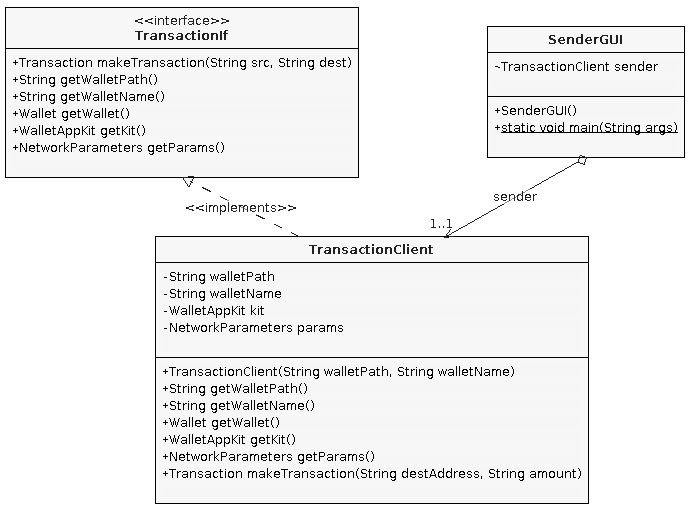
\includegraphics[scale=2]{img/BlockchainCorrect}}
\caption{Diagramma delle classi del Transaction Client}
\label{f:integr:trxclient}
\end{figure}

Il \textit{Transaction Manager} è lo strato software in cui vengono implementate tutte le funzioni di gestione del meccanismo di ricezione dei soldi e restituzione dei dati. 

Il Transaction Manager che si trova all'interno del nodo Server del GRIDS System è composto dalle seguenti classi Java:

\begin{itemize}
    \item TrxManager:
    \item SIoTBitcoinClient:
    \item WalletWrapper:
    \item TransactionResource:
\end{itemize}

Cascata di codice e diagrammi!

\section{Interfacce grafiche ???????}
\label{c:integr:gui}

Aggiungere screenshot della GUI


\section{Casi d'uso}
\label{c:integr:useCase}

Mettere l'acquisto lento, la ricarica, e l'acquisto veloce


ALTRO:

- dire del problema che bisogna aspettare la conferma delle trx di volta in volta, quindi si è pensato di velocizzare l'acquisto dei dati con metodo "a ricarica".

- mettere il sito https://testnet.blockchain.info/ in cui è possibile vedere tutti i blocchi della blockchain in tempo reale
\newpage

%%%%%%%%%%%%%%%%%%%%%%%%%%%%%%%%%%%%%%%%%%%%%%%%%%%%%%%%%%%%%%%%%%%%%%%%%%%%%%%%%%%%%%%%

\chapter{Valutazione delle performance}
\label{c:eval}
Una volta concluso lo sviluppo del GRIDS System con Blockchain integrata, è indispensabile valutarne le performance.
Per fare ciò, bisogna selezionare una metrica appropriata...


È stato misurato il tempo che intercorre tra il momento in cui il client effettua la richiesta di data e quello in cui la transazione viene confermata e l'utente può visualizzare i dati.

Una considerazione molto importante da fare è che, nel caso delle transazioni "lente", vi è una sorta di problema di "campionamento": visto che nella Testnet i blocchi vengono estratti ogni circa 20 minuti, il tempo di ritardo varierà in base a quanto tempo prima è stato risolto l'ultimo blocco della blockchain.

Ho provato con 100 transazioni standard e alcune di esse sono state respinte per "error 64: too-long-mempool-chain": non entravano più nel mempool perché ha una misura limitata! Vedere https://www.mycryptopedia.com/mempool-ex plained/ per la spiegazione.

In Bitcoin Core\footnote{https://bitcoin.org/en/bitcoin-core/} il limite di transazioni non confermate che si possono generare di seguito è 25, quindi pazienza. Con bitcoinj non è stato implementato ancora un modo per aggirare questo limite, avrebbe addirittura poco senso, dato che il fatto che i nodi siano in modalità SPV va in antitesi con il fatto di poter generare un numero molto grande di transazioni.

Però in ogni caso la piattaforma ha il meccanismo recharge, quindi il problema non si pone...

Un'altra importante precisazione da fare è che il mempool error si può verificare quando è un singolo wallet a generare troppe transazioni di seguito, non quando sono tanti wallet a generare meno transazioni: ciò significa che la rete SIoT non costituisce \textit{bottleneck}. In condizioni di utilizzo normale da parte di un utente qualsiasi, difficilmente saranno mandate così tante richieste...
%%

Provare con 25 trx "lente"

Poi con 100 trx "veloci" (fatto)

E poi vediamo i tre grafici: ritardo client-side delle trx standard, ritardo totale delle trx standard, ritardo totale delle transazioni veloci.


\begin{figure}[h!t]
\centerline{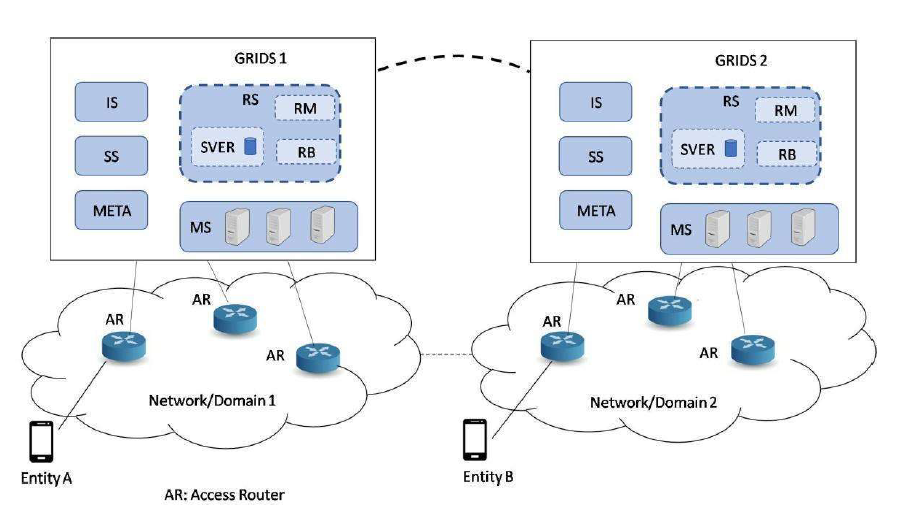
\includegraphics[scale=0.5]{img/GRIDSarch}}
\caption{Architettura del GRIDS System}
\label{f:grids:arch}
\end{figure}
\newpage

%%%%%%%%%%%%%%%%%%%%%%%%%%%%%%%%%%%%%%%%%%%%%%%%%%%%%%%%%%%%%%%%%%%%%%%%%%%%%%%%%%%%%%%

\chapter{Conclusioni e sviluppi futuri}
\label{c:end}
In questo lavoro di tesi è stato ...

Sviluppi futuri:
\begin{itemize}
    \item deployare il sistema nella rete vera dei Bitcoin (con soldi veri!);
    \item fare una blockchain from scratch;
    \item usare altre blockchain (Ethereum, Ripple)
    \item aggiungere gli Smart Contracts
\end{itemize}
\newpage

%%%%%%%%%%%%%%%%%%%%%%%%%%%%%%%%%%%%%%%%%%%%%%%%%%%%%%%%%%%%%%%%%%%%%%%%%%%%%%%%%%%%%%%

%\chapter*{Ringraziamenti}
%\label{chap:Ringraziamenti}
%? la dedica basta e avanza
%\newpage

\addcontentsline{toc}{chapter}{References}
\addcontentsline{toc}{chapter}{Indice Analitico}
\bibliographystyle{ieeetr}
\bibliography{biblio}

\printindex

\end{document}
